\documentclass[a4paper]{article}

\usepackage{color}
\usepackage{graphicx}
\usepackage[normalem]{ulem}

\title{\textbf{Improved Vision and Scope Document}\\\large Requirements Engineering\\Group 42, SA: Tessa Schlief}

\author{Jos Vroegindeweij\\\texttt{s4776755} \and Wouter van Battum\\\texttt{s1011825}
\and Jaap Dijkstra\\\texttt{s4793048}}

\date{\today}

\begin{document}
\maketitle
\color{black}
\section{Product Vision and Business Requirements}
\subsection*{Business Requirements}
\subsubsection*{Background}
This project is about Seats and More. \color{blue}Seats and More started out as a single store with unique products with each its own story. It has now grown to a chain of 8 furniture stores, \color{black}with 8 physical stores in or near larger cities throughout the Netherlands. \color{blue} The aim is still to offer unique products in their stores. \color{black} The philosophy of Seats and More is that furniture should not be bought online: customers should be able to see, touch and test a chair, sofa, table or bed before deciding whether to buy it or not. \color{blue} The managers of the Seats and More store are the only ones invested in the furniture chain, no outside investors are involved. \color{black}

\subsubsection*{Business opportunities}
Seats and More has suggested an application that runs either on customers phones or phones available at the store that can navigate the customers through the store in a personalized manner while also recommending products to the customer, focusing on the products that they are interested in. This will allow clients to find the products they specifically are looking for faster and waste less time on products they are not interested in. Additionally, Seats and More suggested a product reviews system that customers can look at while shopping. It was also suggested to potentially bring customers together with a similar interest in products to further share their experiences on the products. This would allow customers to make a more weighted decision towards purchasing a product in the Seats and More store.

\subsubsection*{Business Objectives}
The main ambition of Seats and More is to create a shopping experience that will please a growing group of returning customers. Seats and More hopes to attract both customers who still buy their furniture at physical stores as well as customers who are already used at buying furniture online. The main objective is to have a 15\% increase in revenue after the first year. \sout{The other objectives are as follows:}
\begin{itemize}
\item \sout{Let the customers be navigated in a personalized manner through the store, focusing on the products that they are interested in, while avoiding congestions due to too many customers in a small area of the store.}
\item \sout{Let the customers be recommended products based on their interests. Should a particular product be sold out, an alternative product should be recommended to the customer.}
\item \sout{Provide the customers with product reviews or let them review a product themselves. These might be the reviews of all customers in the same physical store, or the reviews of all customers of all 8 physical stores.}
\item \sout{Let the customers create a wish list or shopping cart and then take the decision to buy the selected products via the website.}
\item \sout{BO-1: Attract 30 \% more old (customers that already used to come to the physical store) within 12 months.}
\item \sout{BO-2: Attract 50 \% new customers that used to shop for furniture online within 12 months.}
\item \sout{BO-3: Increase sales by 40 \% within 6 months.}
\end{itemize}

\subsubsection*{Success Metrics}
The success of the changes is measured by an increased number of satisfied customers, customers that have tested the furniture before buying it instead of only having seen a picture, \color{blue}and customers that have stated that the shopping experience is better than shopping online. \color{black}Seats and More also wants that these changes as a result of an increased number of satisfied customers result in less returned items.

\subsubsection*{Vision Statement}
For customers who want to buy furniture, the new product information system is an information system that will navigate the customers through the store in a personalized manner. The system also recommends the customers products based on their interests, and should a product be sold out, an alternative product should be recommended. This system should provide product reviews that the customers can read (or listen to) or provide themselves. The system should also have a wish list or shopping cart for customers to add selected products and make the decision to buy them via the website. Unlike the current way customers can buy furniture at online stores, where the customers cannot see, touch and test furniture. Our product will create a shopping experience as pleasant and personalized as possible.

\subsubsection*{Business Risks}
There are a few risks for Seats and More if they implement new the product information system. Due to software errors, Seats and More risk having congestions in the store. If the customers are not navigated the proper way, congestions can occur and that is what Seats and More wants to avoid. 
Seats and More risk having smart phones/and or tablet stolen. If the customers picked up a smart phone or tablet at the entrance and they do not return them that could cost Seats and More a lot of money when it happens often. 
Another risk is that customers don not want to come to a store and then have to buy their furniture online. 
Customers don not want to put in too much of an effort, so they might lose customers over this.

\subsubsection*{Business Assumptions and Dependencies}
\begin{itemize}
\item Assumptions
\end{itemize}
Seats and More assumed that customers only want to see products that they are interested in, and not just look around in the store and see everything Seats and More has.
Seats and More assume that customers want to be recommended about other products.
They also assume that customers are willing to travel further distances to see the furniture, because eight stores throughout the Netherlands is not much.

\begin{itemize}
\item Dependencies
\end{itemize}
Seats and More is dependent on customers actually wanting to test and see the furniture they buy. Most web shops these days allow a customer to view a piece of furniture in the relevant room on their smartphone.
Seats and More is also dependent on the software engineers. If the software for the app is implemented wrongly, then for examples congestions can occur or customers could be sent to the wrong furniture in the store.

We have come to conclusion that Seats and More is a company with big opportunities to grow and expand her clientele. Using this chapter, we are able to create the scope and limitations and business context of Seats and More.


\section{Scope and limitations}
\subsection*{Major features}
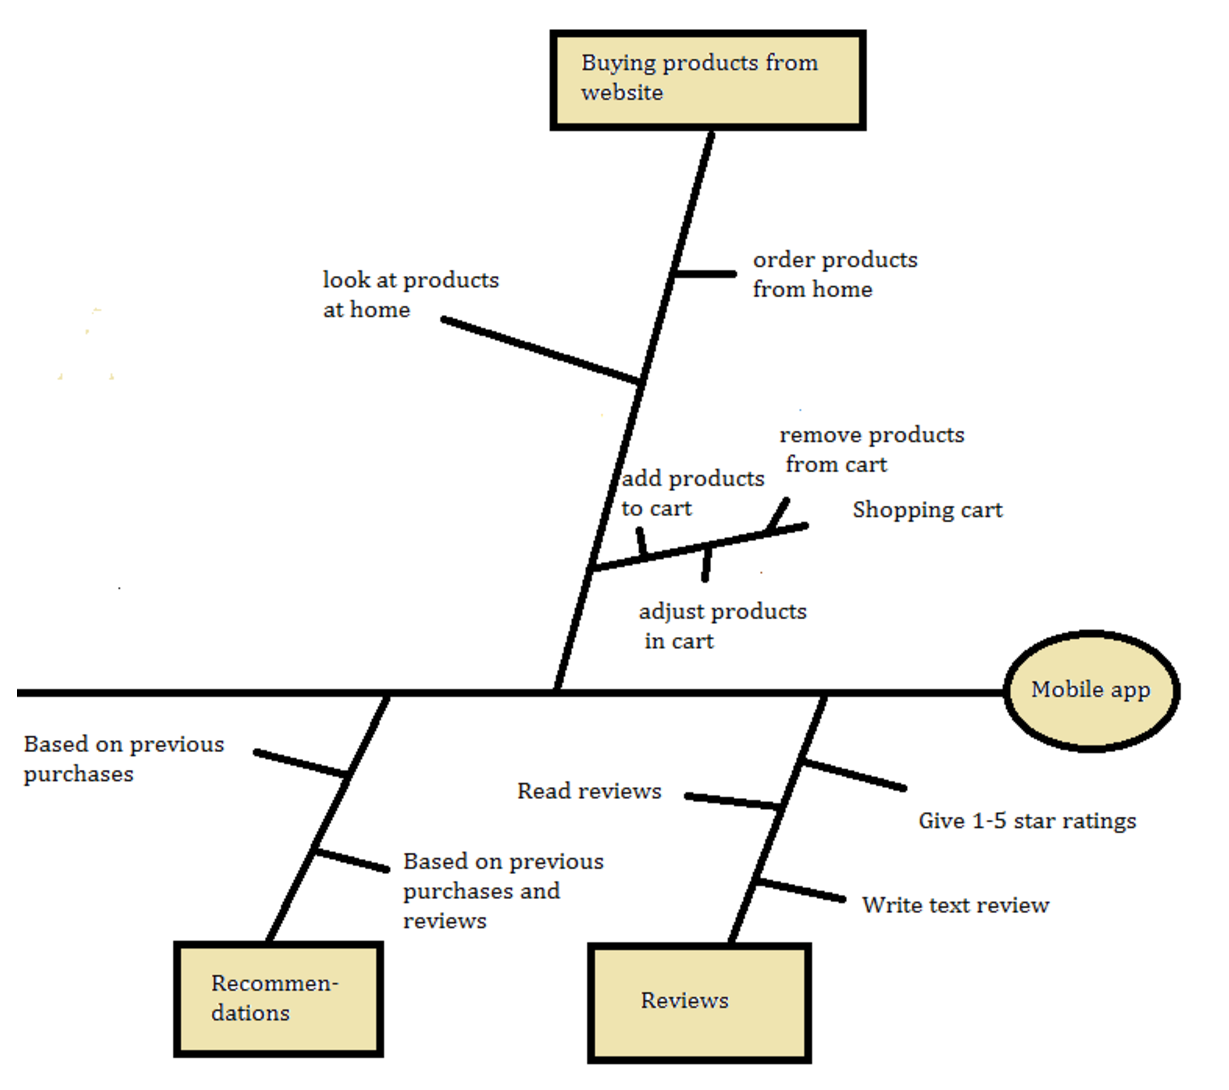
\includegraphics[scale=0.7]{new_feature_tree.eps}
\begin{itemize}
\item FE 1: \sout{Customers will be navigated through the store in a personalized manner, in such a way that there won't be congestions by having too many customers in the same area.}
\item FE 2: Writing and reading product reviews
\item FE 3: Give recommendations to customers based on previous purchases and written reviews
\item FE 4: Placing products in shopping cart and buying them from a website at home.
\end{itemize}

Features that will \textbf{not} be implemented:
\begin{itemize}
\item \color{blue} Customers will be navigated through the store in a personalized manner, in such a way that there won't be congestions by having too many customers in the same area.

\item Customers can \textit{listen} to reviews.\color{black}

\item Bringing customers that are interested in the same products together to drink a cup of coffee.
\item Having the app integrated with in-store physical objects.
\end{itemize}

\subsection*{Scope of initial and subsequent releases}
\color{blue}As discussed with the management of \textit{Seats and More}, instead of having multiple subsequent releases, the focus will be entirely on the initial release of the system. The features implemented in this release will therefore be the major features discussed in the \textit{Major Features} section of this document.\color{black}
\subsection*{Limitations and exclusions}
\color{blue}The personalized route through the store is seen as less of a priority in the eyes of the management than the other major features and therefore will not be implemented.\\
\\
Listening to reviews has been rejected by the management because the management does not like seeing people walk around the store with headphones on.\\
\\
Bringing customers that are interested in the same products together to drink coffee will not be done as the majority of the management does not support the implementation of this feature.\\\color{black}
\\
Using in-store objects to communicate with the app is infeasible and will therefore not be implemented.

\section{Business Context}
\subsection*{Stakeholder profiles}
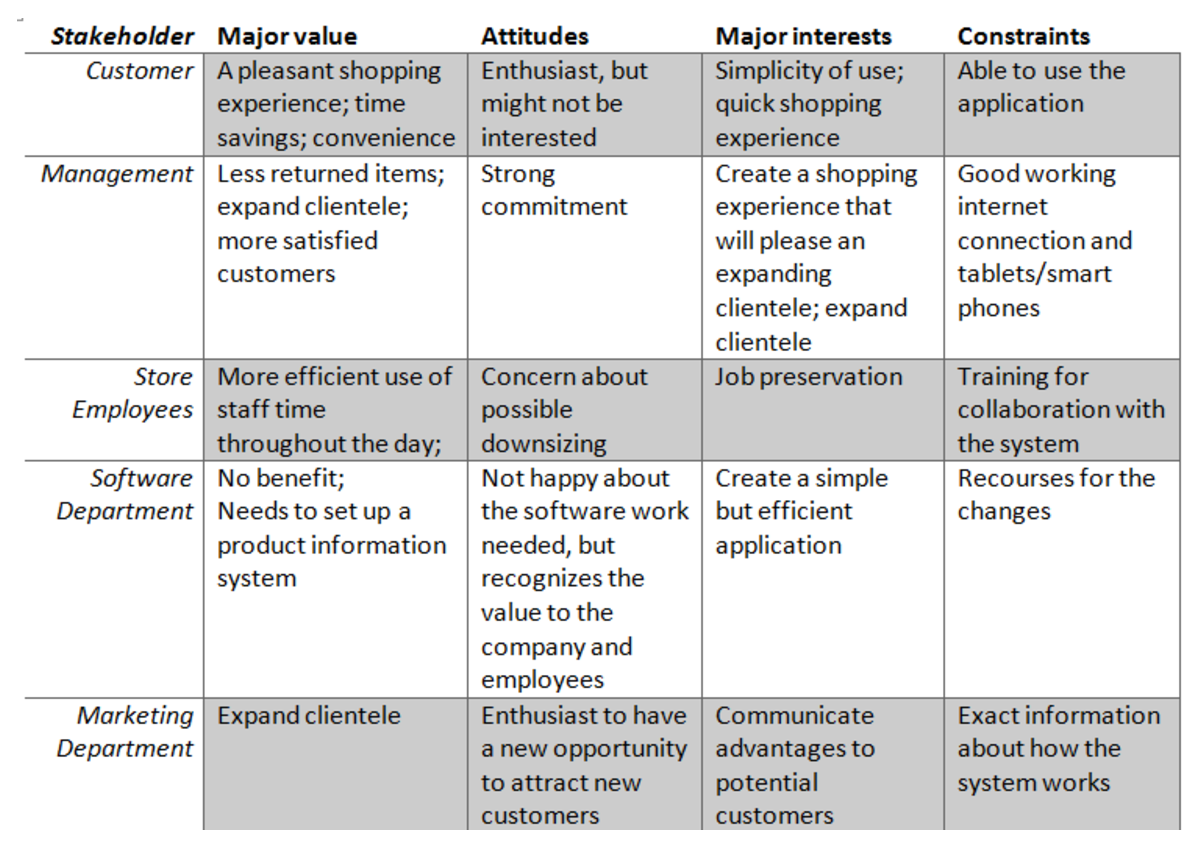
\includegraphics[scale=0.7]{stakeholder_profiles.eps}

\subsection*{Project priority}
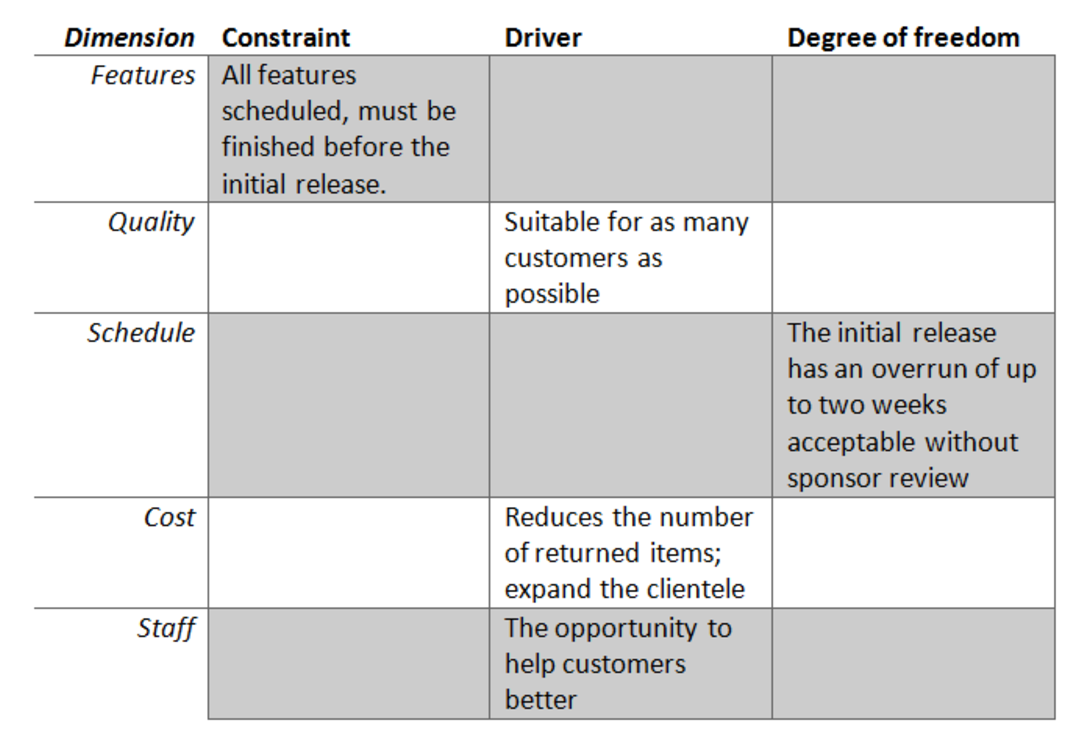
\includegraphics[scale=0.9]{project_priority.eps}

\subsection*{Deployment considerations}
The internet surfer must be upgraded to handle the increased usage of the internet by all the smartphones or tablets. The app has to be developed for different operating systems, such as iOS, Android or Windows Phone or tablet. Any infrastructure changes must be in place before the initial release. The customer database must have enough storage to store the preferences of the customers and the shopping cart. The store’s staff must get training to help them work with the new system and because of that will be able to help customers better.\\
\\
We have come to the conclusion that there are a lot of things to keep in mind and take into account when making the new product information system. 



\end{document}